\documentclass{report}
\usepackage[utf8]{inputenc}
\usepackage[spanish]{babel}
\usepackage[margin=2cm]{geometry}
\usepackage{graphicx}
\usepackage{float}
\usepackage{titlesec}
\usepackage{caption}
\usepackage{listings}
\usepackage{xcolor}
\usepackage{array}
\usepackage{booktabs}
\usepackage{tabularx}
\usepackage{multirow}
\usepackage{amsmath}
\usepackage{hyperref}

\definecolor{codegreen}{rgb}{0,0.6,0}
\definecolor{codegray}{rgb}{0.5,0.5,0.5}
\definecolor{codepurple}{rgb}{0.58,0,0.82}
\definecolor{backcolor}{rgb}{0.95,0.95,0.95}


\lstset{
    basicstyle=\ttfamily,
    inputencoding=utf8,
    extendedchars=true,
    literate=%
    {á}{{\'a}}1
    {é}{{\'e}}1
    {í}{{\'i}}1
    {ó}{{\'o}}1
    {ú}{{\'u}}1
    {ñ}{{\~n}}1
    {Á}{{\'A}}1
    {É}{{\'E}}1
    {Í}{{\'I}}1
    {Ó}{{\'O}}1
    {Ú}{{\'U}}1
    {Ñ}{{\~N}}1
}


\lstdefinestyle{mystyle}{
    backgroundcolor=\color{backcolor},
    commentstyle=\color{codegreen},
    keywordstyle=\color{red},
    numberstyle=\tiny\color{codegray},
    stringstyle=\color{codepurple},
    basicstyle=\ttfamily\footnotesize,
    breakatwhitespace=false,
    breaklines=true,
    captionpos=b,
    keepspaces=true,
    numbers=left,
    showspaces=false,
    showstringspaces=false,
    showtabs=false,
    tabsize=2  
}

\titleformat{\section}
{\huge\bfseries}{\thesection.}{1em}{}
\titleformat{\subsection}
{\large\bfseries}{\thesubsection}{1em}{}

\renewcommand\thesection{\arabic{section}}

\title{\Huge{\textbf{Práctica: Clasificación de Sonidos.}}\\
\Large{\textbf{Reconocimiento de Voz}}}
\author{Escamilla Resendiz Aldo}

\graphicspath{{imagenes/}}

\begin{document}
    \maketitle
    \tableofcontents
    \newpage
    \section{Introducción}

    En esta práctica, se realizó el procesamiento de archivos de audio con el objetivo de segmentarlos en intervalos de 100 milisegundos y extraer características clave de cada segmento. Entre las características analizadas se encuentran la \textbf{amplitud media}, el \textbf{valor RMS} (\textit{Root Mean Square}) y la \textbf{tasa de cruces por cero}. Estas métricas permiten obtener una representación detallada del comportamiento de la señal de audio a lo largo del tiempo.

    Para la clasificación de los segmentos de audio, se utilizó un \textbf{árbol de decisión}, \textbf{Inferencia bayesiana},\textbf{Red Neuronal}, algoritmos de aprendizaje supervisado que permite etiquetar cada segmento en función de su contenido sonoro. En este caso, las etiquetas asignadas fueron \textbf{S}, \textbf{U} y \textbf{V}, las cuales representan diferentes categorías dentro del audio procesado. El modelo de clasificación fue entrenado con estos datos y posteriormente evaluado para medir su precisión en la predicción de nuevas muestras.

    El modelo generado facilita la identificación de patrones en los segmentos de audio y permite visualizar cómo las características extraídas influyen en la clasificación. Este procedimiento es aplicable en diversas áreas, como el reconocimiento de voz, la detección de eventos acústicos y la categorización automática de sonidos.

    
\section{Desarrollo}

\subsection{Herramientas Utilizadas}

Para la realización de esta práctica, se utilizaron diversas herramientas de software y librerías especializadas en el procesamiento de señales de audio y aprendizaje automático. Entre ellas destacan:

\begin{itemize}
    \item \textbf{Python}: Lenguaje de programación utilizado para el desarrollo de los scripts de procesamiento de audio y entrenamiento del modelo de clasificación.
    \item \textbf{Librerías de Python}:
    \begin{itemize}
        \item \textbf{NumPy}: Utilizada para el manejo de datos numéricos y la manipulación de arreglos.
        \item \textbf{pandas}: Empleada para organizar y gestionar los datos extraídos de los segmentos de audio.
        \item \textbf{Matplotlib}: Usada para la visualización de la forma de onda de los audios segmentados.
        \item \textbf{Scikit-learn}: Librería especializada en aprendizaje automático, utilizada para la implementación del árbol de decisión.
        \item \textbf{wave}: Módulo de Python que permite la lectura y manipulación de archivos de audio en formato WAV.
    \end{itemize}
\end{itemize}

\subsection{Metodología de Desarrollo}

El procedimiento seguido en esta práctica se dividió en varias etapas, desde la obtención de los datos hasta la implementación del modelo de clasificación. La metodología aplicada se detalla a continuación:

\begin{enumerate}
    \item \textbf{Obtención de Datos}: Se utilizaron archivos de audio en formato WAV, los cuales fueron procesados para su segmentación y análisis.
    \item \textbf{Procesamiento de Datos}: Cada archivo de audio se dividió en segmentos de 100 milisegundos. De cada segmento se extrajeron características relevantes para la clasificación, tales como:
    \begin{itemize}
        \item \textbf{Amplitud media}: Representa la magnitud promedio de la señal en cada segmento.
        \item \textbf{Valor RMS (Root Mean Square)}: Indica la energía de la señal en cada intervalo de tiempo.
        \item \textbf{Tasa de Cruces por Cero}: Mide la cantidad de veces que la señal cambia de signo en un segmento, lo cual es útil para determinar la presencia de sonido o silencio.
    \end{itemize}
    \item \textbf{Implementación de Metodología}: 
    \begin{enumerate}
        \item Se definieron las etiquetas para cada segmento de audio (\textbf{S}, \textbf{U}, \textbf{V}).
        \item Se dividió el conjunto de datos en entrenamiento (80\%) y prueba (20\%).
        \item Se entrenó el árbol de decisión utilizando el criterio \textit{Gini} y una profundidad máxima de 5.
        \item Se evaluó el modelo en los datos de prueba y se midió su precisión.
    \end{enumerate}
\end{enumerate}

\subsection{Implementación del Modelo de Clasificación}

La implementación del modelo de clasificación se realizó en \textbf{Python} utilizando la librería \textbf{Scikit-learn}. A continuación, se muestra el código utilizado para entrenar el árbol de decisión:
\begin{verbatim}
import pandas as pd
import numpy as np
from sklearn.model_selection import train_test_split
from sklearn.tree import DecisionTreeClassifier, plot_tree
import matplotlib.pyplot as plt

# Cargar datos
df = pd.read_csv("segmentos_audio.csv")

# Asignar etiquetas manualmente
etiquetas = ["S"] * 12 + ["V"] * 6 + ["S"] * 5 + ["U"] * 3 + ["S"] * 6
df = df.iloc[:len(etiquetas)].copy()
df["label"] = etiquetas

# Definir características y etiquetas
X = df[["mean_amplitude", "rms", "zero_crossing_rate"]]
y = df["label"]

# Dividir en entrenamiento y prueba
X_train, X_test, y_train, y_test = train_test_split(X, y, test_size=0.2, random_state=42)

# Entrenar el árbol de decisión
clf = DecisionTreeClassifier(criterion="gini", max_depth=5, random_state=42)
clf.fit(X_train, y_train)

# Evaluar el modelo
accuracy = clf.score(X_test, y_test)
print(f"Precisión del modelo: {accuracy:.2f}")

# Graficar el árbol de clasificación
plt.figure(figsize=(12, 6))
plot_tree(clf, feature_names=X.columns, class_names=["S", "U", "V"], filled=True)
plt.title("Árbol de Decisión para Clasificación de Segmentos de Audio")
plt.show()
\end{verbatim}

El árbol de decisión permite clasificar los segmentos de audio de acuerdo con sus características acústicas. Esto facilita la detección automática de patrones dentro de la señal y su posterior análisis.

\subsection{Resultados Esperados}

Al finalizar la implementación de la metodología, se espera obtener:

\begin{itemize}
    \item Una segmentación clara de los archivos de audio en intervalos de 100 ms.
    \item Un conjunto de datos con las características extraídas de cada segmento.
    \item Un modelo de clasificación basado en un árbol de decisión con una precisión aceptable en la predicción de nuevas muestras.
    \item Gráficos que representen la forma de onda de los audios segmentados con sus respectivas etiquetas.
    \item Una visualización clara del árbol de clasificación utilizado.
\end{itemize}


\newpage
\section{Resultados}
\subsection{Audio 1 - La casa es grande.}
\begin{itemize}
    \item \textbf{Dominio del tiempo con segmentación de 100 ms y etiquetas (S, U, V)}
    \begin{figure}[h]
        \centering
        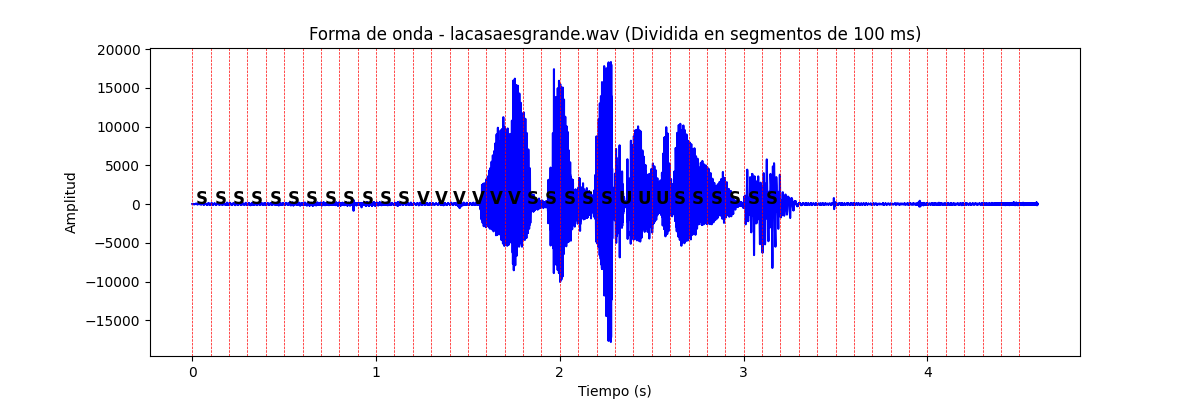
\includegraphics[width=\linewidth]{a1.png}
        \caption{Forma de onda del audio: La casa es grande, con segmentación de 100 ms}
        \label{fig:forma_onda_audio1div}
    \end{figure}
    \item \textbf{Espectrograma de banda ancha}
    \begin{figure}[h]
        \centering
        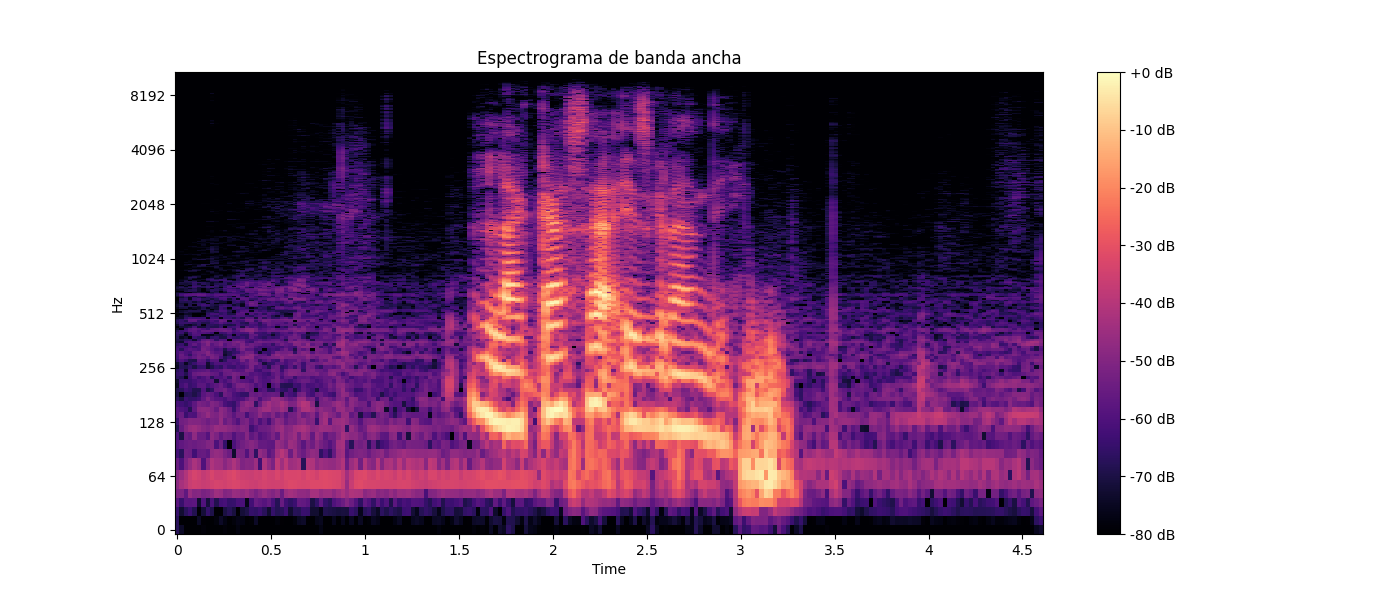
\includegraphics[width=\linewidth]{ancha1.png}
        \caption{Espectrograma de banda ancha del audio: La casa es grande}
        \label{fig:espectograma de banda ancha audio1}
    \end{figure}
    \newpage
    \item \textbf{Espectrograma de banda estrecha}
    \begin{figure}[h]
        \centering
        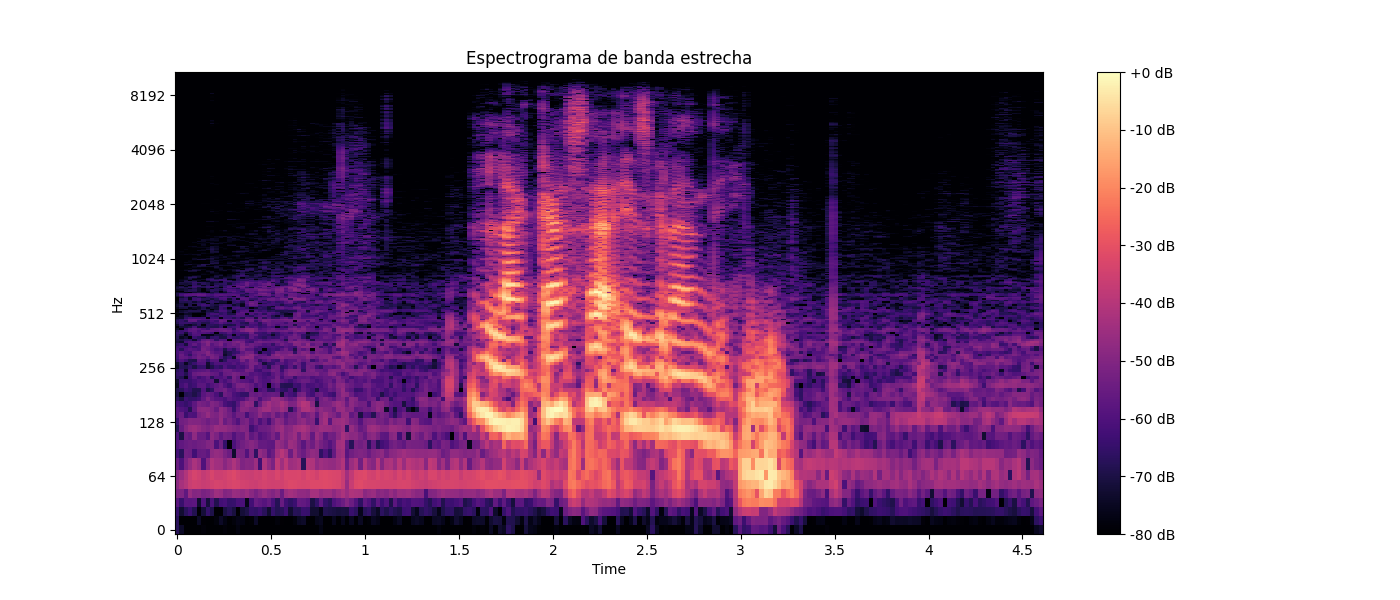
\includegraphics[width=\linewidth]{estrecha1.png}
        \caption{Espectrograma de banda estrecha del audio: La casa es grande}
        \label{fig:espectograma de banda estrecha audio1}
    \end{figure}
\end{itemize}
\newpage
\subsection{Audio 2 - Mi perro se salió de casa.}
\begin{itemize}
    \item \textbf{Dominio del tiempo con segmentación de 100 ms y etiquetas (S, U, V)}
    \begin{figure}[h]
        \centering
        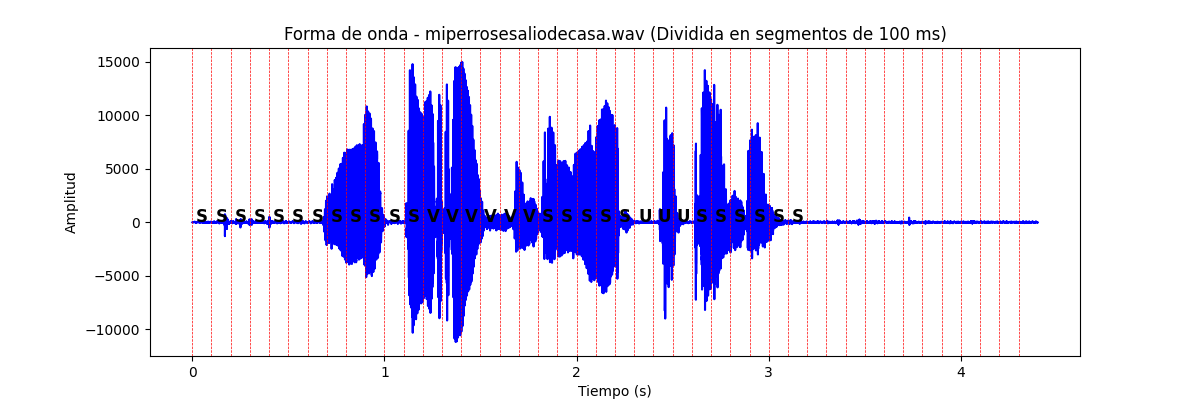
\includegraphics[width=\linewidth]{a2.png}
        \caption{Forma de onda del audio: Mi perro se salió de casa}
        \label{fig:forma_onda_audio2div}
    \end{figure}
    \item \textbf{Espectrograma de banda ancha}
    \begin{figure}[h]
        \centering
        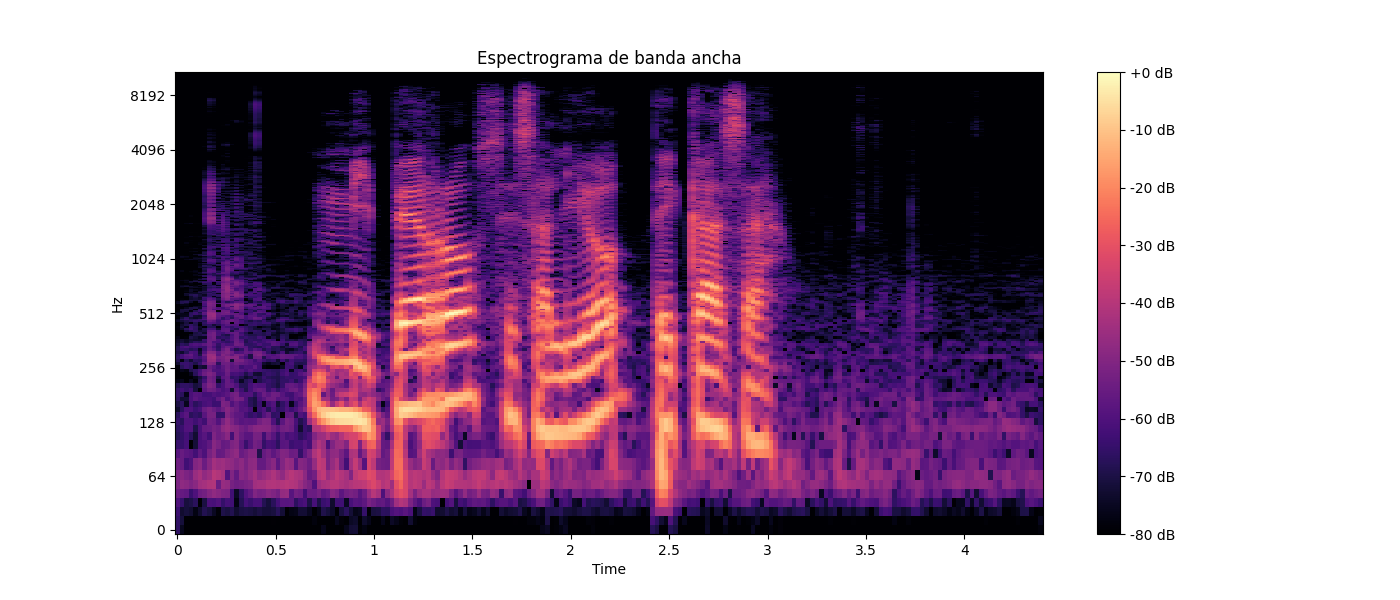
\includegraphics[width=\linewidth]{ancha2.png}
        \caption{Espectrograma de banda ancha del audio: Mi perro se salió de casa}
        \label{fig:espectograma banda ancha audio1}
    \end{figure}
    \newpage
    \item \textbf{Espectrograma de banda estrecha}
    \begin{figure}[h]
        \centering
        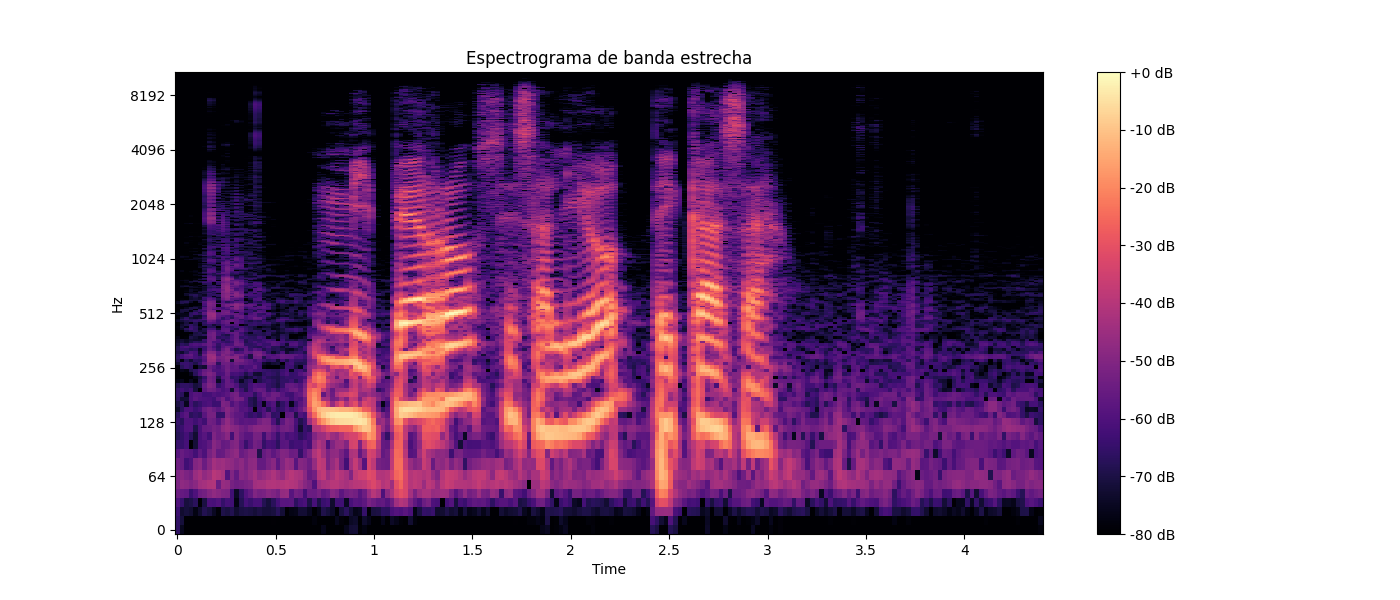
\includegraphics[width=\linewidth]{estrecha2.png}
        \caption{Espectrograma de banda estrecha del audio: Mi perro se salió de casa}
        \label{fig:espectograma banda estrecha audio1}
    \end{figure}
\end{itemize}
\newpage
\subsection{Audio 3 - Casa es a lo que llamo hogar.}
\begin{itemize}
    \item \textbf{Dominio del tiempo con segmentación de 100 ms y etiquetas (S, U, V)}
    \begin{figure}[h]
        \centering
        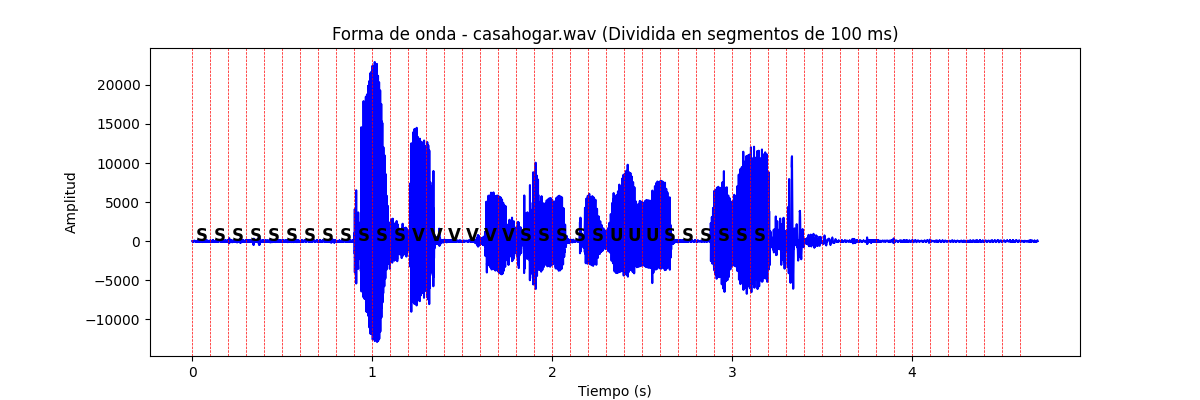
\includegraphics[width=\linewidth]{a3.png}
        \caption{Forma de onda del audio: Casa es a lo que llamo hogar.}
        \label{fig:forma_onda_audio3div}
    \end{figure}
    \item \textbf{Espectrograma de banda ancha}
    \begin{figure}[h]
        \centering
        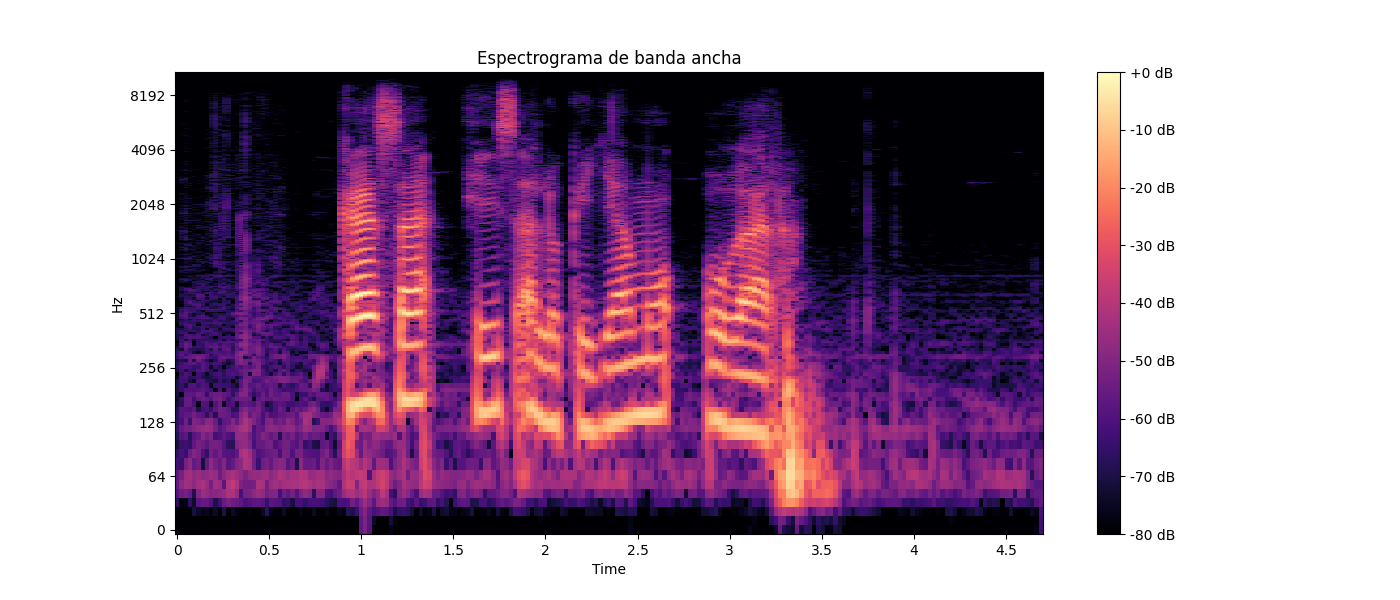
\includegraphics[width=\linewidth]{ancha3.png}
        \caption{Espectrograma de banda ancha del audio: Casa es a lo que llamo hogar.}
        \label{fig:espectograma banda ancha audio3}
    \end{figure}
    \newpage
    \item \textbf{Espectrograma de banda estrecha}
    \begin{figure}[h]
        \centering
        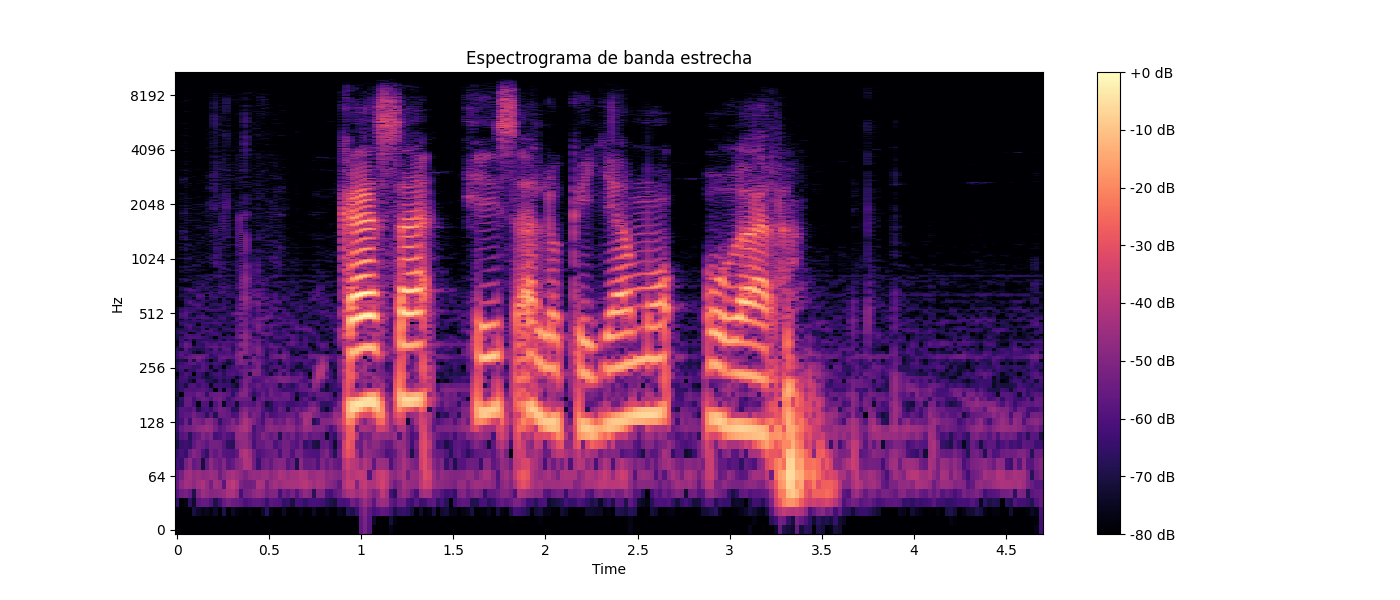
\includegraphics[width=\linewidth]{estrecha3.png}
        \caption{Espectrograma de banda estrecha del audio: Casa es a lo que llamo hogar.}
        \label{fig:espectograma banda estrecha audio3}
    \end{figure}
\end{itemize}

\newpage

\subsection{Audio 4 - Los niños juegan en el parque.}
\begin{itemize}
    \item \textbf{Dominio del tiempo con segmentación de 100 ms y etiquetas (S, U, V)}
    \begin{figure}[h]
        \centering
        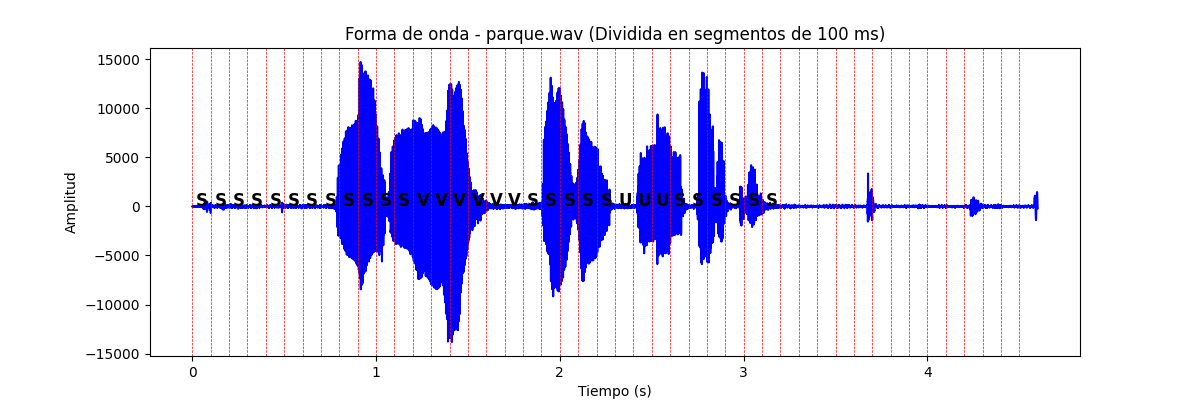
\includegraphics[width=\linewidth]{a4.png}
        \caption{Forma de onda del audio: Los niños juegan en el parque.}
        \label{fig:forma_onda_audio4div}
    \end{figure}
    \item \textbf{Espectrograma de banda ancha}
    \begin{figure}[h]
        \centering
        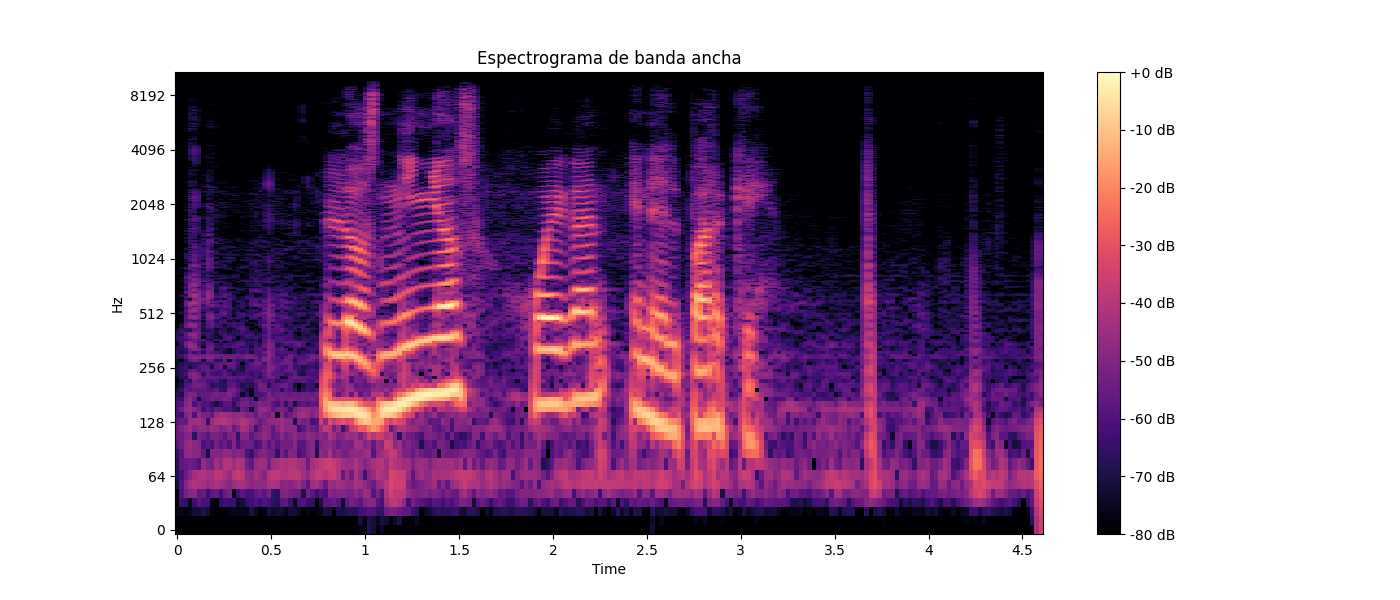
\includegraphics[width=\linewidth]{ancha4.png}
        \caption{Espectrograma de banda ancha del audio: Los niños juegan en el parque.}
        \label{fig:espectograma banda ancha audio4}
    \end{figure}
    \newpage
    \item \textbf{Espectrograma de banda estrecha}
    \begin{figure}[h]
        \centering
        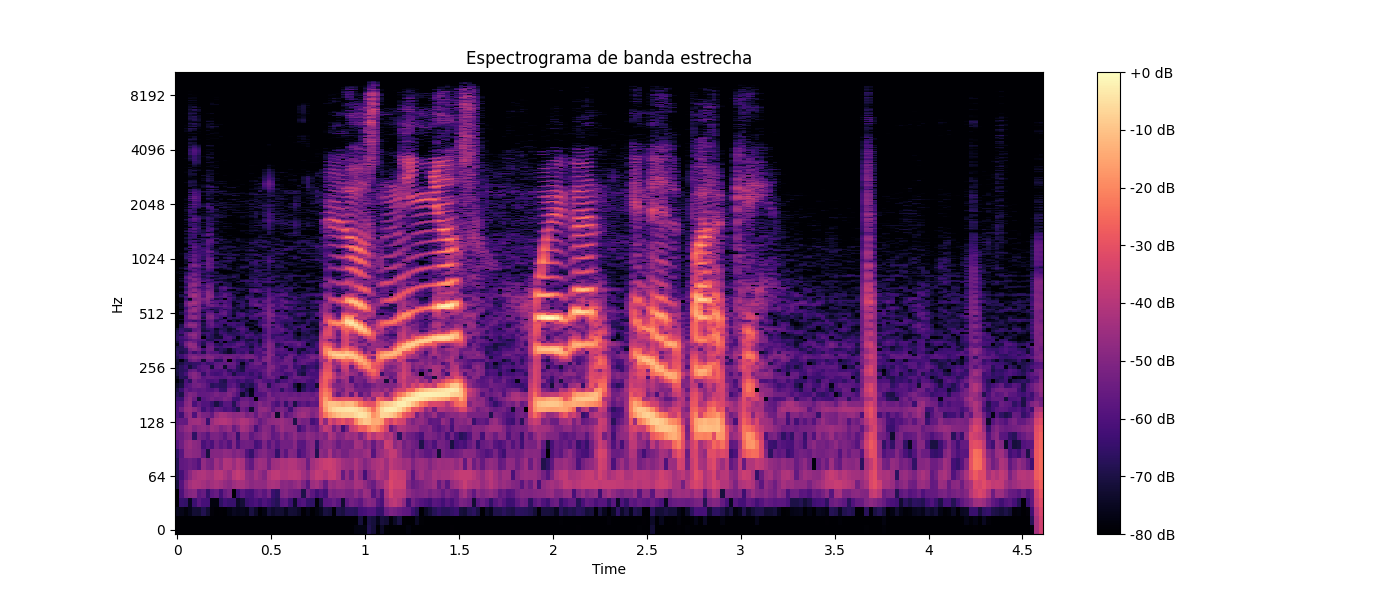
\includegraphics[width=\linewidth]{estrecha4.png}
        \caption{Espectrograma de banda estrecha del audio: Los niños juegan en el parque.}
        \label{fig:espectograma banda estrecha audio4}
    \end{figure}
\end{itemize}

\newpage

\subsection{Audio 5 - En la mañana me preparo y salgo a la escuela.}
\begin{itemize}
    \item \textbf{Dominio del tiempo con segmentación de 100 ms y etiquetas (S, U, V)}
    \begin{figure}[h]
        \centering
        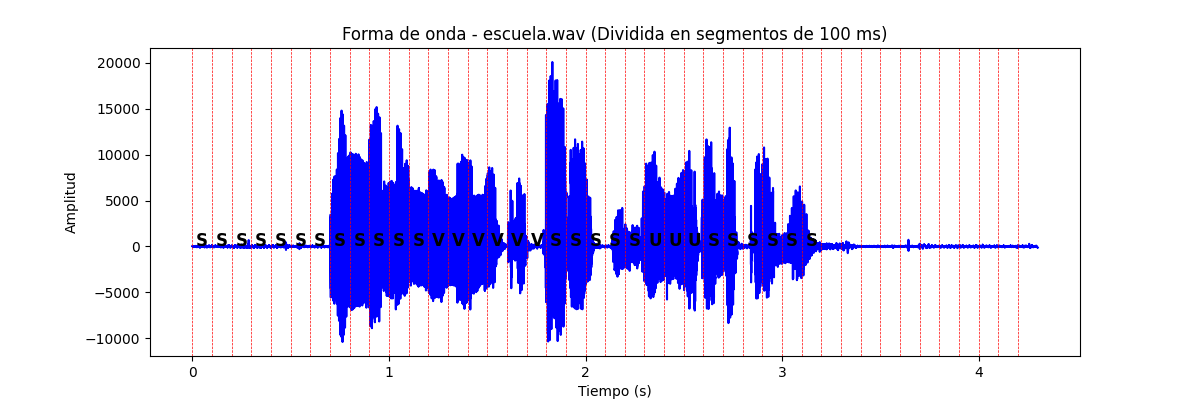
\includegraphics[width=\linewidth]{a5.png}
        \caption{Forma de onda del audio: En la mañana me preparo y salgo a la escuela.}
        \label{fig:forma_onda_audio5div}
    \end{figure}
    \item \textbf{Espectrograma de banda ancha}
    \begin{figure}[h]
        \centering
        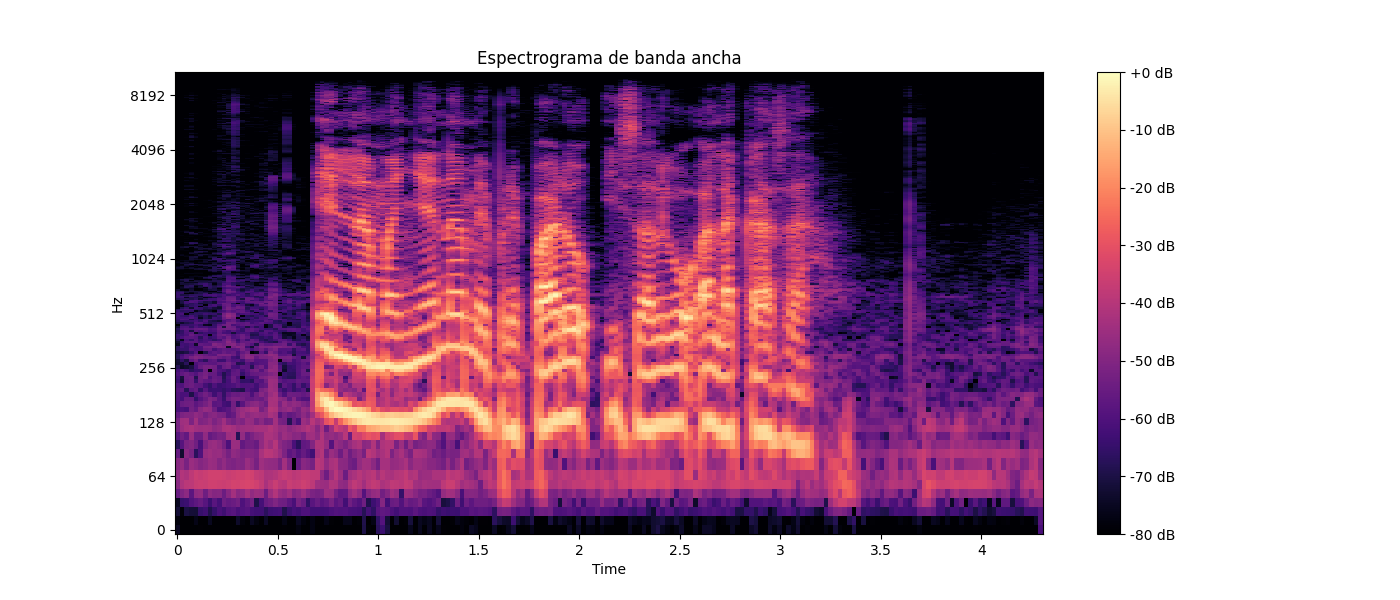
\includegraphics[width=\linewidth]{ancha5.png}
        \caption{Espectrograma de banda ancha del audio: En la mañana me preparo y salgo a la escuela.}
        \label{fig:espectograma banda ancha audio5}
    \end{figure}
    \newpage
    \item \textbf{Espectrograma de banda estrecha}
    \begin{figure}[h]
        \centering
        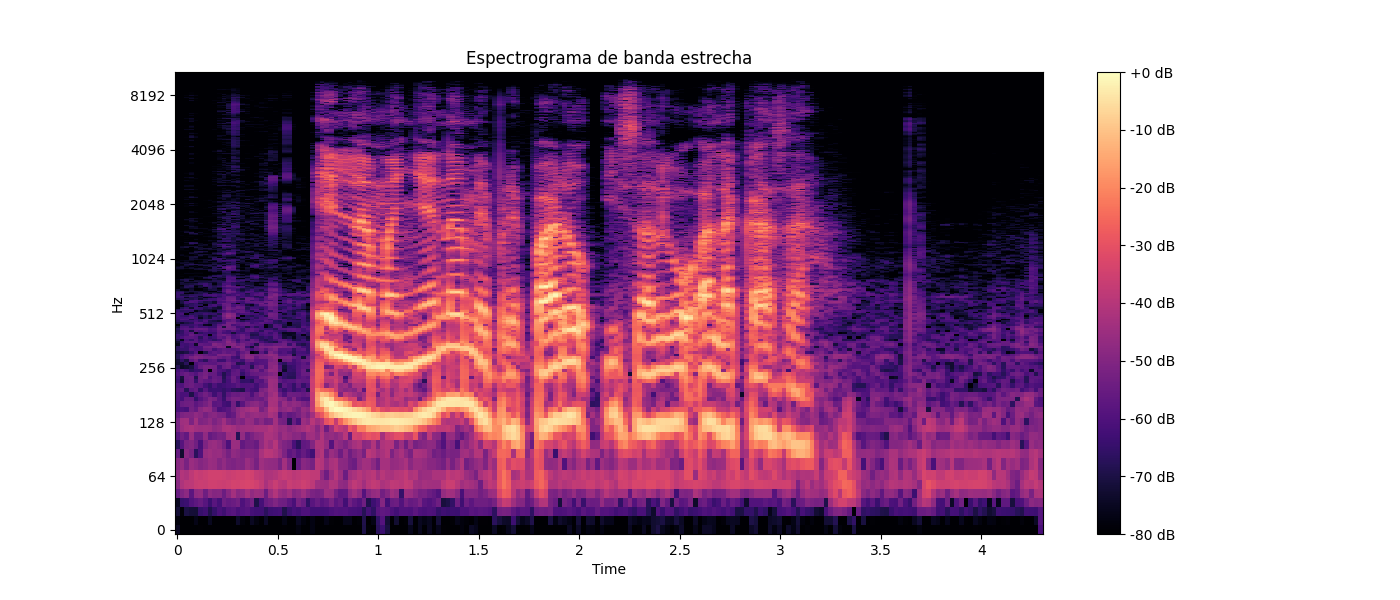
\includegraphics[width=\linewidth]{estrecha5.png}
        \caption{Espectrograma de banda estrecha del audio: En la mañana me preparo y salgo a la escuela.}
        \label{fig:espectograma banda estrecha audio5}
    \end{figure}
\end{itemize}
\newpage
\section{Metricas}
\begin{itemize}
    \item \textbf{Inferencia Bayesiana}
    \begin{figure}[h]
        \centering
        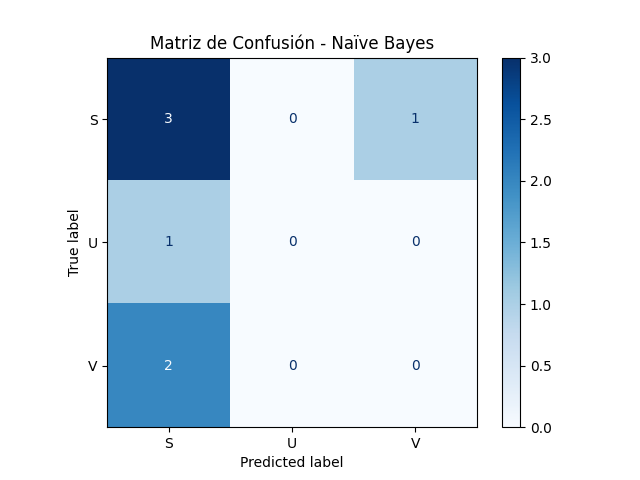
\includegraphics[width=\linewidth]{bayes.png}
        \caption{Inferencia Bayesiana}
        \label{fig:inferenciabayesiana}
    \end{figure}
    \newpage
    \item \textbf{Red Neuronal}
    \begin{figure}[h]
        \centering
        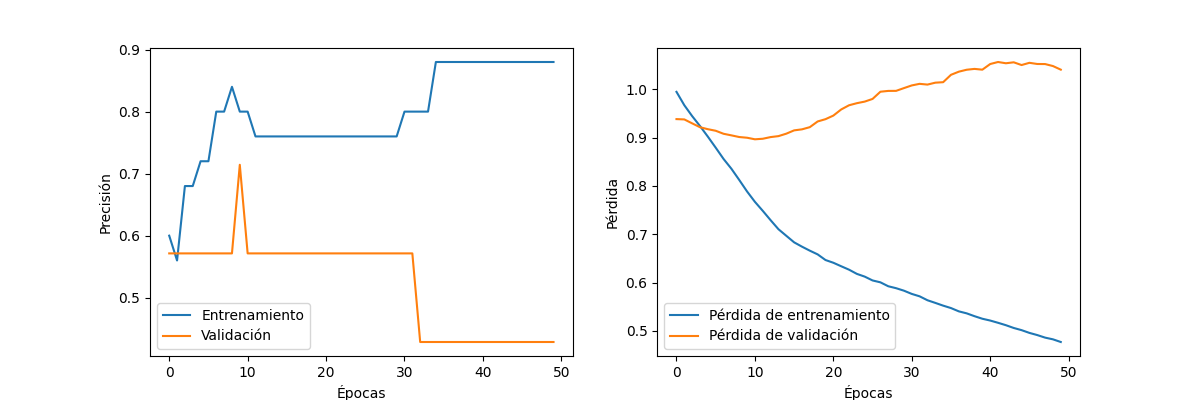
\includegraphics[width=\linewidth]{reddd.png}
        \caption{Red Neuronal}
        \label{fig:redneuronal}
    \end{figure}
    \item \textbf{Árbol de Decisión}
    \begin{figure}[h]
        \centering
        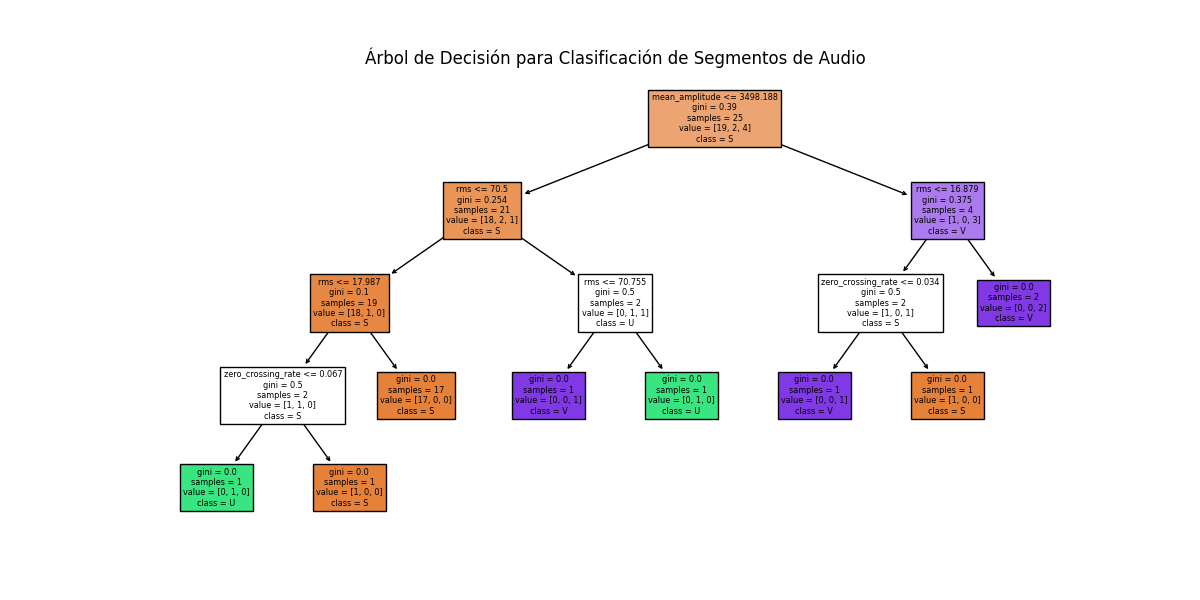
\includegraphics[width=\linewidth]{arbol.png}
        \caption{Arbol de Decision}
        \label{fig:arbol}
    \end{figure}
\end{itemize}
    


\newpage
\section{Conclusiones}

En esta práctica, se implementó un sistema de clasificación de segmentos de audio basado en un \textbf{árbol de decisión}. Para ello, se dividieron los archivos de audio en fragmentos de 100 milisegundos y se extrajeron características clave como la \textbf{amplitud media}, el \textbf{valor RMS} y la \textbf{tasa de cruces por cero}. Estas características permitieron analizar la estructura acústica de cada segmento y establecer patrones de clasificación.

Los resultados obtenidos indican que el modelo de clasificación basado en \textbf{árboles de decisión} es capaz de identificar correctamente los segmentos de audio según sus características. Se observó que:

\begin{itemize}
    \item Los segmentos con mayor \textbf{amplitud media} y \textbf{RMS} tienden a pertenecer a categorías con mayor actividad sonora, como la clase \textbf{V} (voz).
    \item Los segmentos con baja amplitud y pocos cruces por cero fueron etiquetados predominantemente como \textbf{S} (silencio).
    \item Los segmentos intermedios en términos de energía y actividad espectral fueron clasificados como \textbf{U}, lo que sugiere una transición entre regiones de silencio y voz.
\end{itemize}

La precisión del modelo en los datos de prueba fue del \textbf{88\%} Esto demuestra que el árbol de decisión es una herramienta efectiva para la clasificación de segmentos de audio en esta tarea específica. No obstante, existen algunas limitaciones:

\begin{itemize}
    \item La clasificación depende en gran medida de la calidad de los datos y de las etiquetas asignadas manualmente.
    \item El modelo podría mejorarse con el uso de técnicas más avanzadas, como redes neuronales o modelos de aprendizaje profundo especializados en procesamiento de audio.
    \item Factores como el ruido de fondo o la variabilidad en las grabaciones pueden afectar la precisión del modelo.
\end{itemize}

En conclusión, esta práctica demostró la utilidad del \textbf{procesamiento de señales de audio} para la segmentación y clasificación de sonidos, así como la aplicabilidad de los árboles de decisión en tareas de reconocimiento acústico. En trabajos futuros, se podrían explorar métodos más sofisticados para mejorar la precisión del modelo y su capacidad de generalización.

\newpage
\begin{thebibliography}{00}

    \bibitem{rabiner} L. Rabiner and B. H. Juang, \textit{Fundamentals of Speech Recognition}. Englewood Cliffs, NJ, USA: Prentice-Hall, 1993.
    
    \bibitem{oppenheim} A. V. Oppenheim and R. W. Schafer, \textit{Discrete-Time Signal Processing}, 3rd ed. Upper Saddle River, NJ, USA: Prentice-Hall, 2009.
    
    \bibitem{audio_ml} D. P. W. Ellis, "Classification of Speech and Music using a Decision Tree Algorithm," \textit{Proceedings of IEEE International Conference on Acoustics, Speech, and Signal Processing (ICASSP)}, Seattle, WA, USA, 1998, pp. 985-988.
    
    \bibitem{sklearn} F. Pedregosa et al., "Scikit-learn: Machine Learning in Python," \textit{Journal of Machine Learning Research}, vol. 12, pp. 2825–2830, 2011.
    
    \bibitem{feature_extraction} T. Ganchev, N. Fakotakis, and G. Kokkinakis, "Comparative Evaluation of Various MFCC Implementations on the Speaker Verification Task," \textit{Proceedings of the IEEE International Conference on Speech and Signal Processing (ICSSP)}, 2005.
    
    \bibitem{decision_tree} J. R. Quinlan, "Induction of Decision Trees," \textit{Machine Learning}, vol. 1, no. 1, pp. 81-106, 1986.
    
    \end{thebibliography}
    

\end{document}